\begin{fact} \label{quadri}
	Considérons tous les quadrilatères de périmètre fixé $p$. Parmi tous ces quadrilatères, il en existe un seul d'aire maximale, c'est le carré de côté $c = \num{.25} p$.
\end{fact}


\begin{proof}
    Commençons par exclure les quadrilatères avec un angle au sommet rentrant, c'est-à-dire supérieur à l'angle plat. 
    Si tel est le cas, aucun des trois autres angles au sommet ne peut être rentrant, car la somme des quatre angles est $(4 - 2)\pi = 2 \pi$.%
    \footnote{
    	Un quadrilatère $\setproba{Q}$ sans angle rentrant est forcément convexe, c'est-à-dire tel que pour toute paire de points $M$ et $N$ de la surface fermée bornée créée par $\setproba{Q}$, le segment $[MN]$ est dans cette surface.
    }
    Comme dans la figure suivante, pour tout quadrilatère $ABCD$ de périmètre $p$ avec $\anglein{B}$ rentrant, il existe un quadrilatère $AB^{\,\prime}CD$ sans angle rentrant, de périmètre $p$, et tel que $\area{AB^{\,\prime}CD} > \area{ABCD}$.
	Notre recherche doit donc continuer avec des quadrilatères sans angle rentrant, et de périmètre $p$.

	\begin{center}
		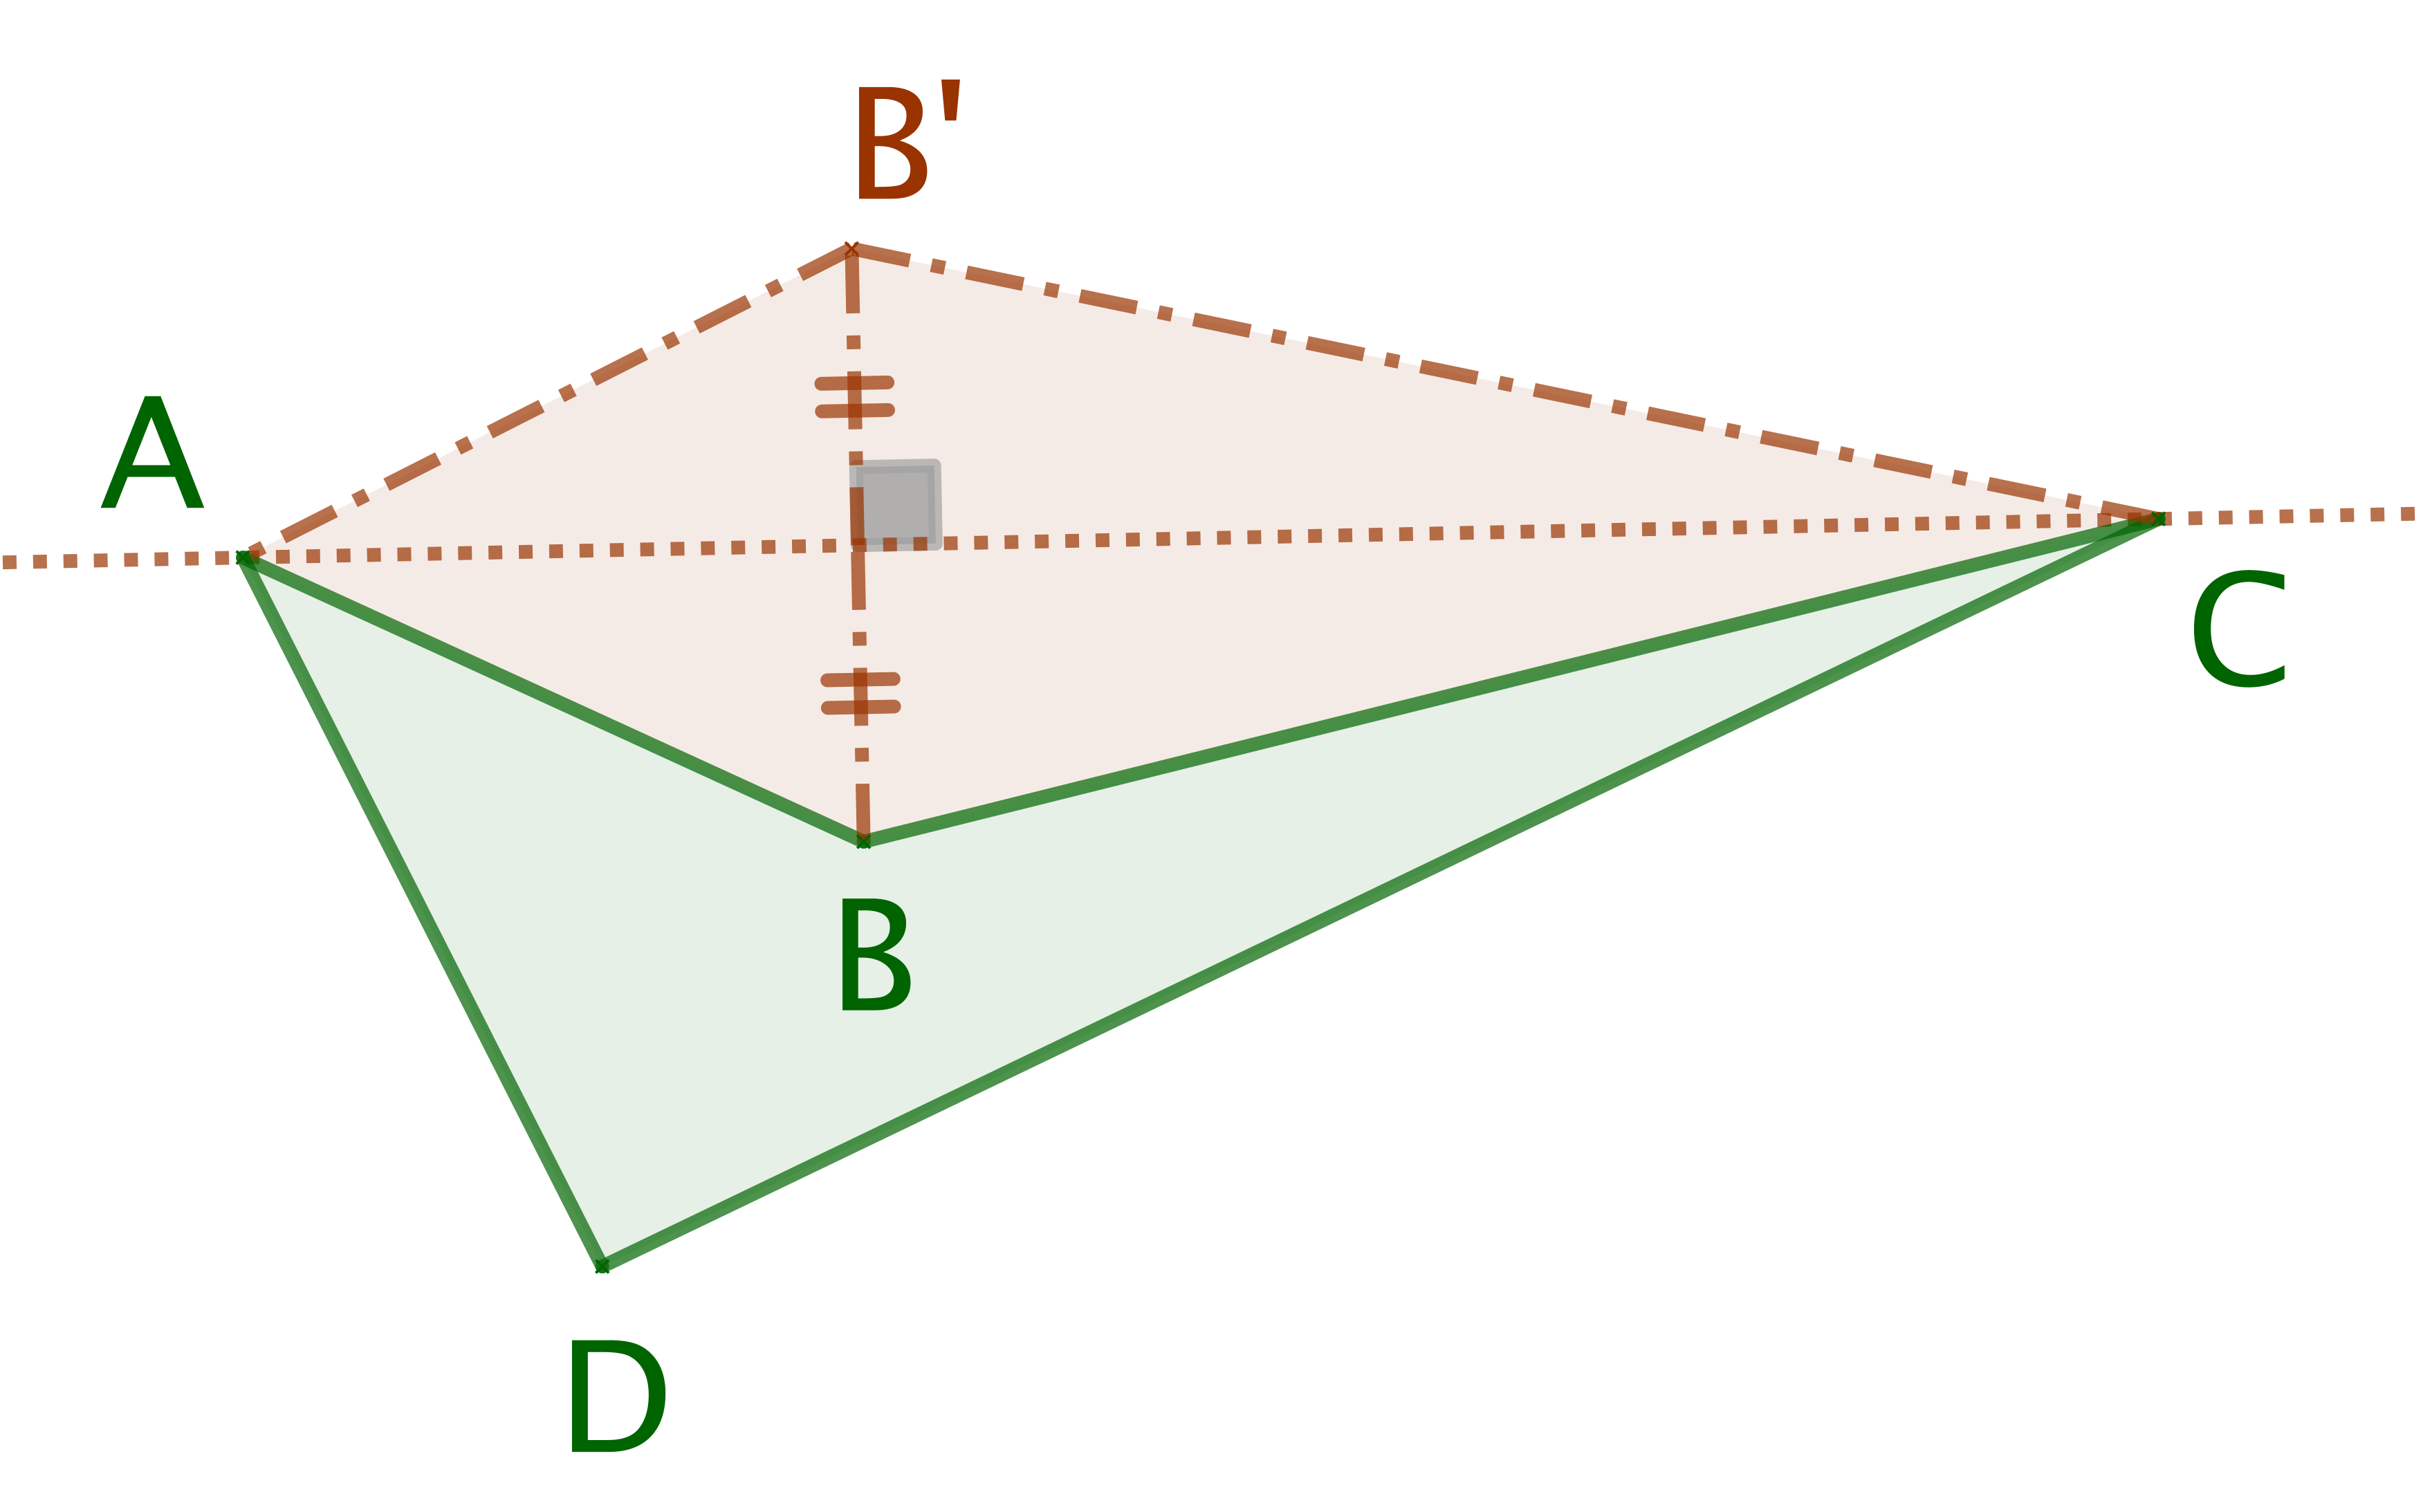
\includegraphics[scale=.4]{non-convex.png}
	\end{center}
	
	
	Si $ABCD$ est sans angle rentrant, de périmètre $p$, et tel que $AB \neq BC$, le fait \ref{tri-one-side-fixed} donne $AB^{\,\prime}CD$ sans angle rentrant, de périmètre $p$,%
	\footnote{
		Noter que
		$\perim{AB^{\,\prime}CD} = \perim{AB^{\,\prime}C} + \perim{ACD} - 2 AC$.
	}
	avec $AB^{\,\prime} = B^{\,\prime}C$ et $\area{AB^{\,\prime}CD} > \area{ABCD}$ comme dans la figure ci-après.
	Nous nous ramenons ainsi au cas d'un quadrilatère $ABCD$ sans angle rentrant, de périmètre $p$, et tel que $AB = BC$.

	\begin{center}
		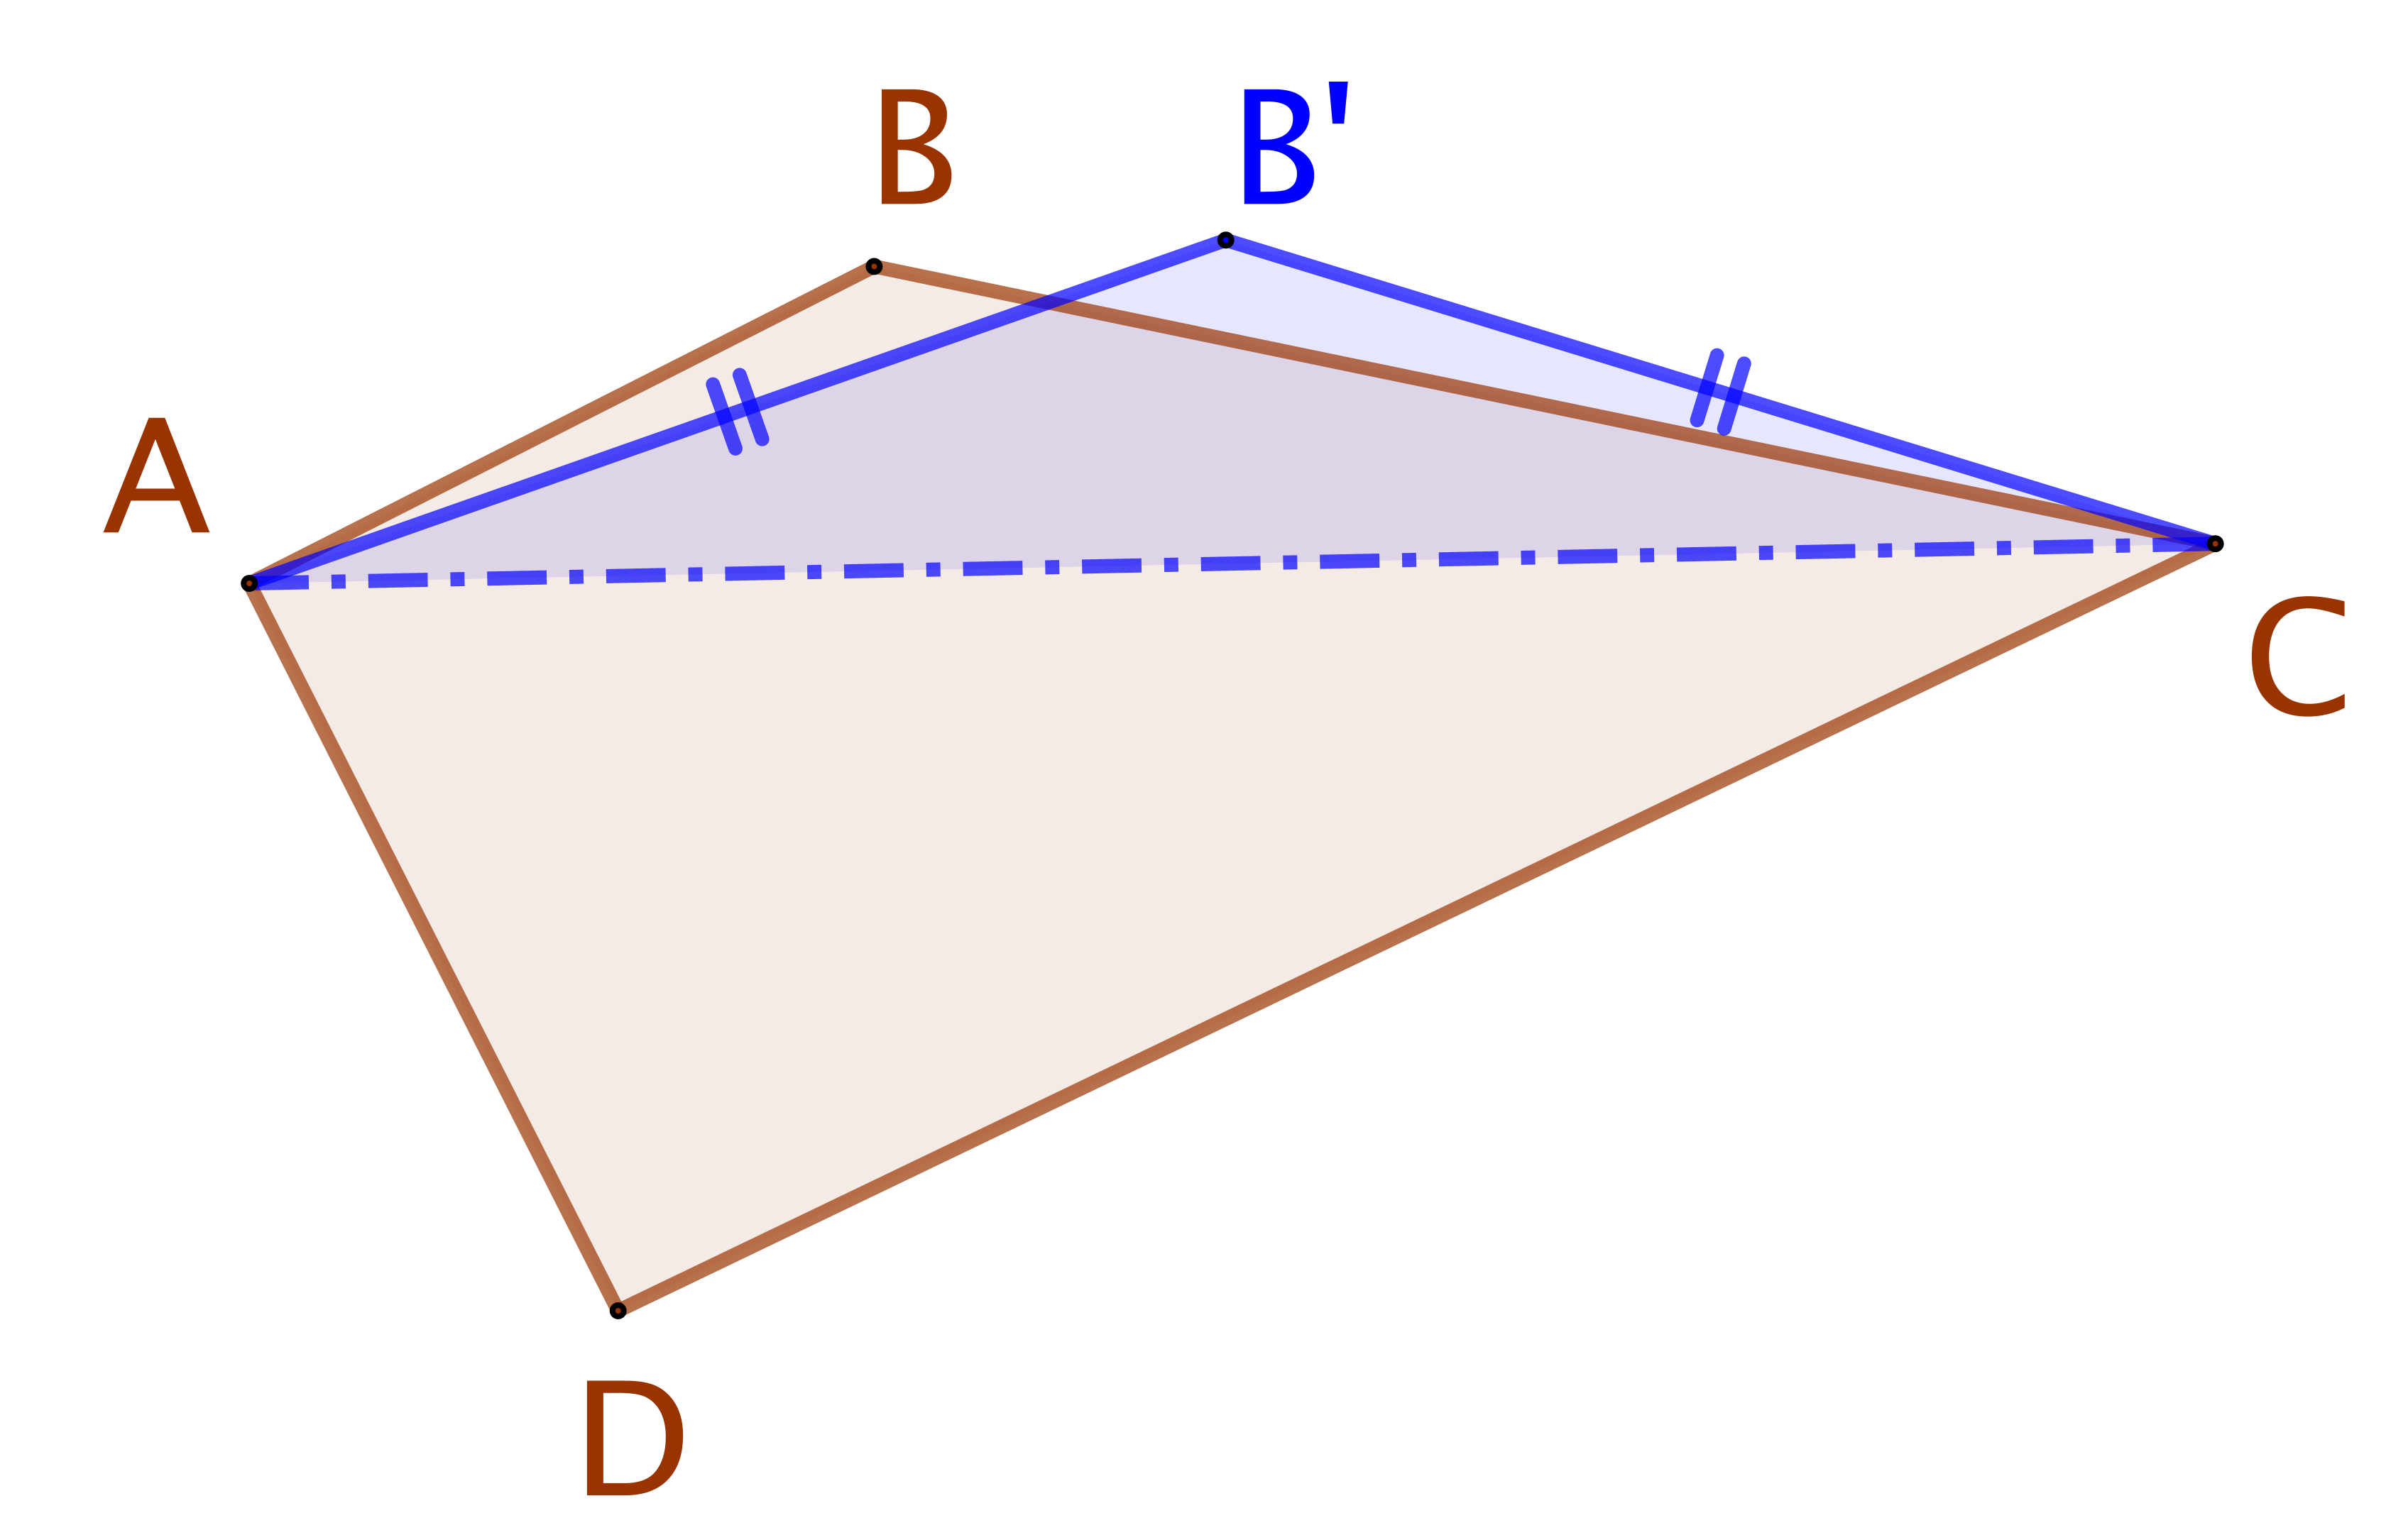
\includegraphics[scale=.4]{convex-gene.png}
	\end{center}
	
	
	La méthode précédente appliquée au sommet $D$ d'un quadrilatère $ABCD$ sans angle rentrant, de périmètre $p$, avec $AB = BC$, mais $AD \neq DC$, permet de se ramener au cas d'un cerf-volant $ABCD$ de périmètre $p$, et de sommets principaux $B$ et $D$, c'est-à-dire tel que $AB = BC$ et $AD = DC$, voir ci-dessous.  

	\begin{center}
		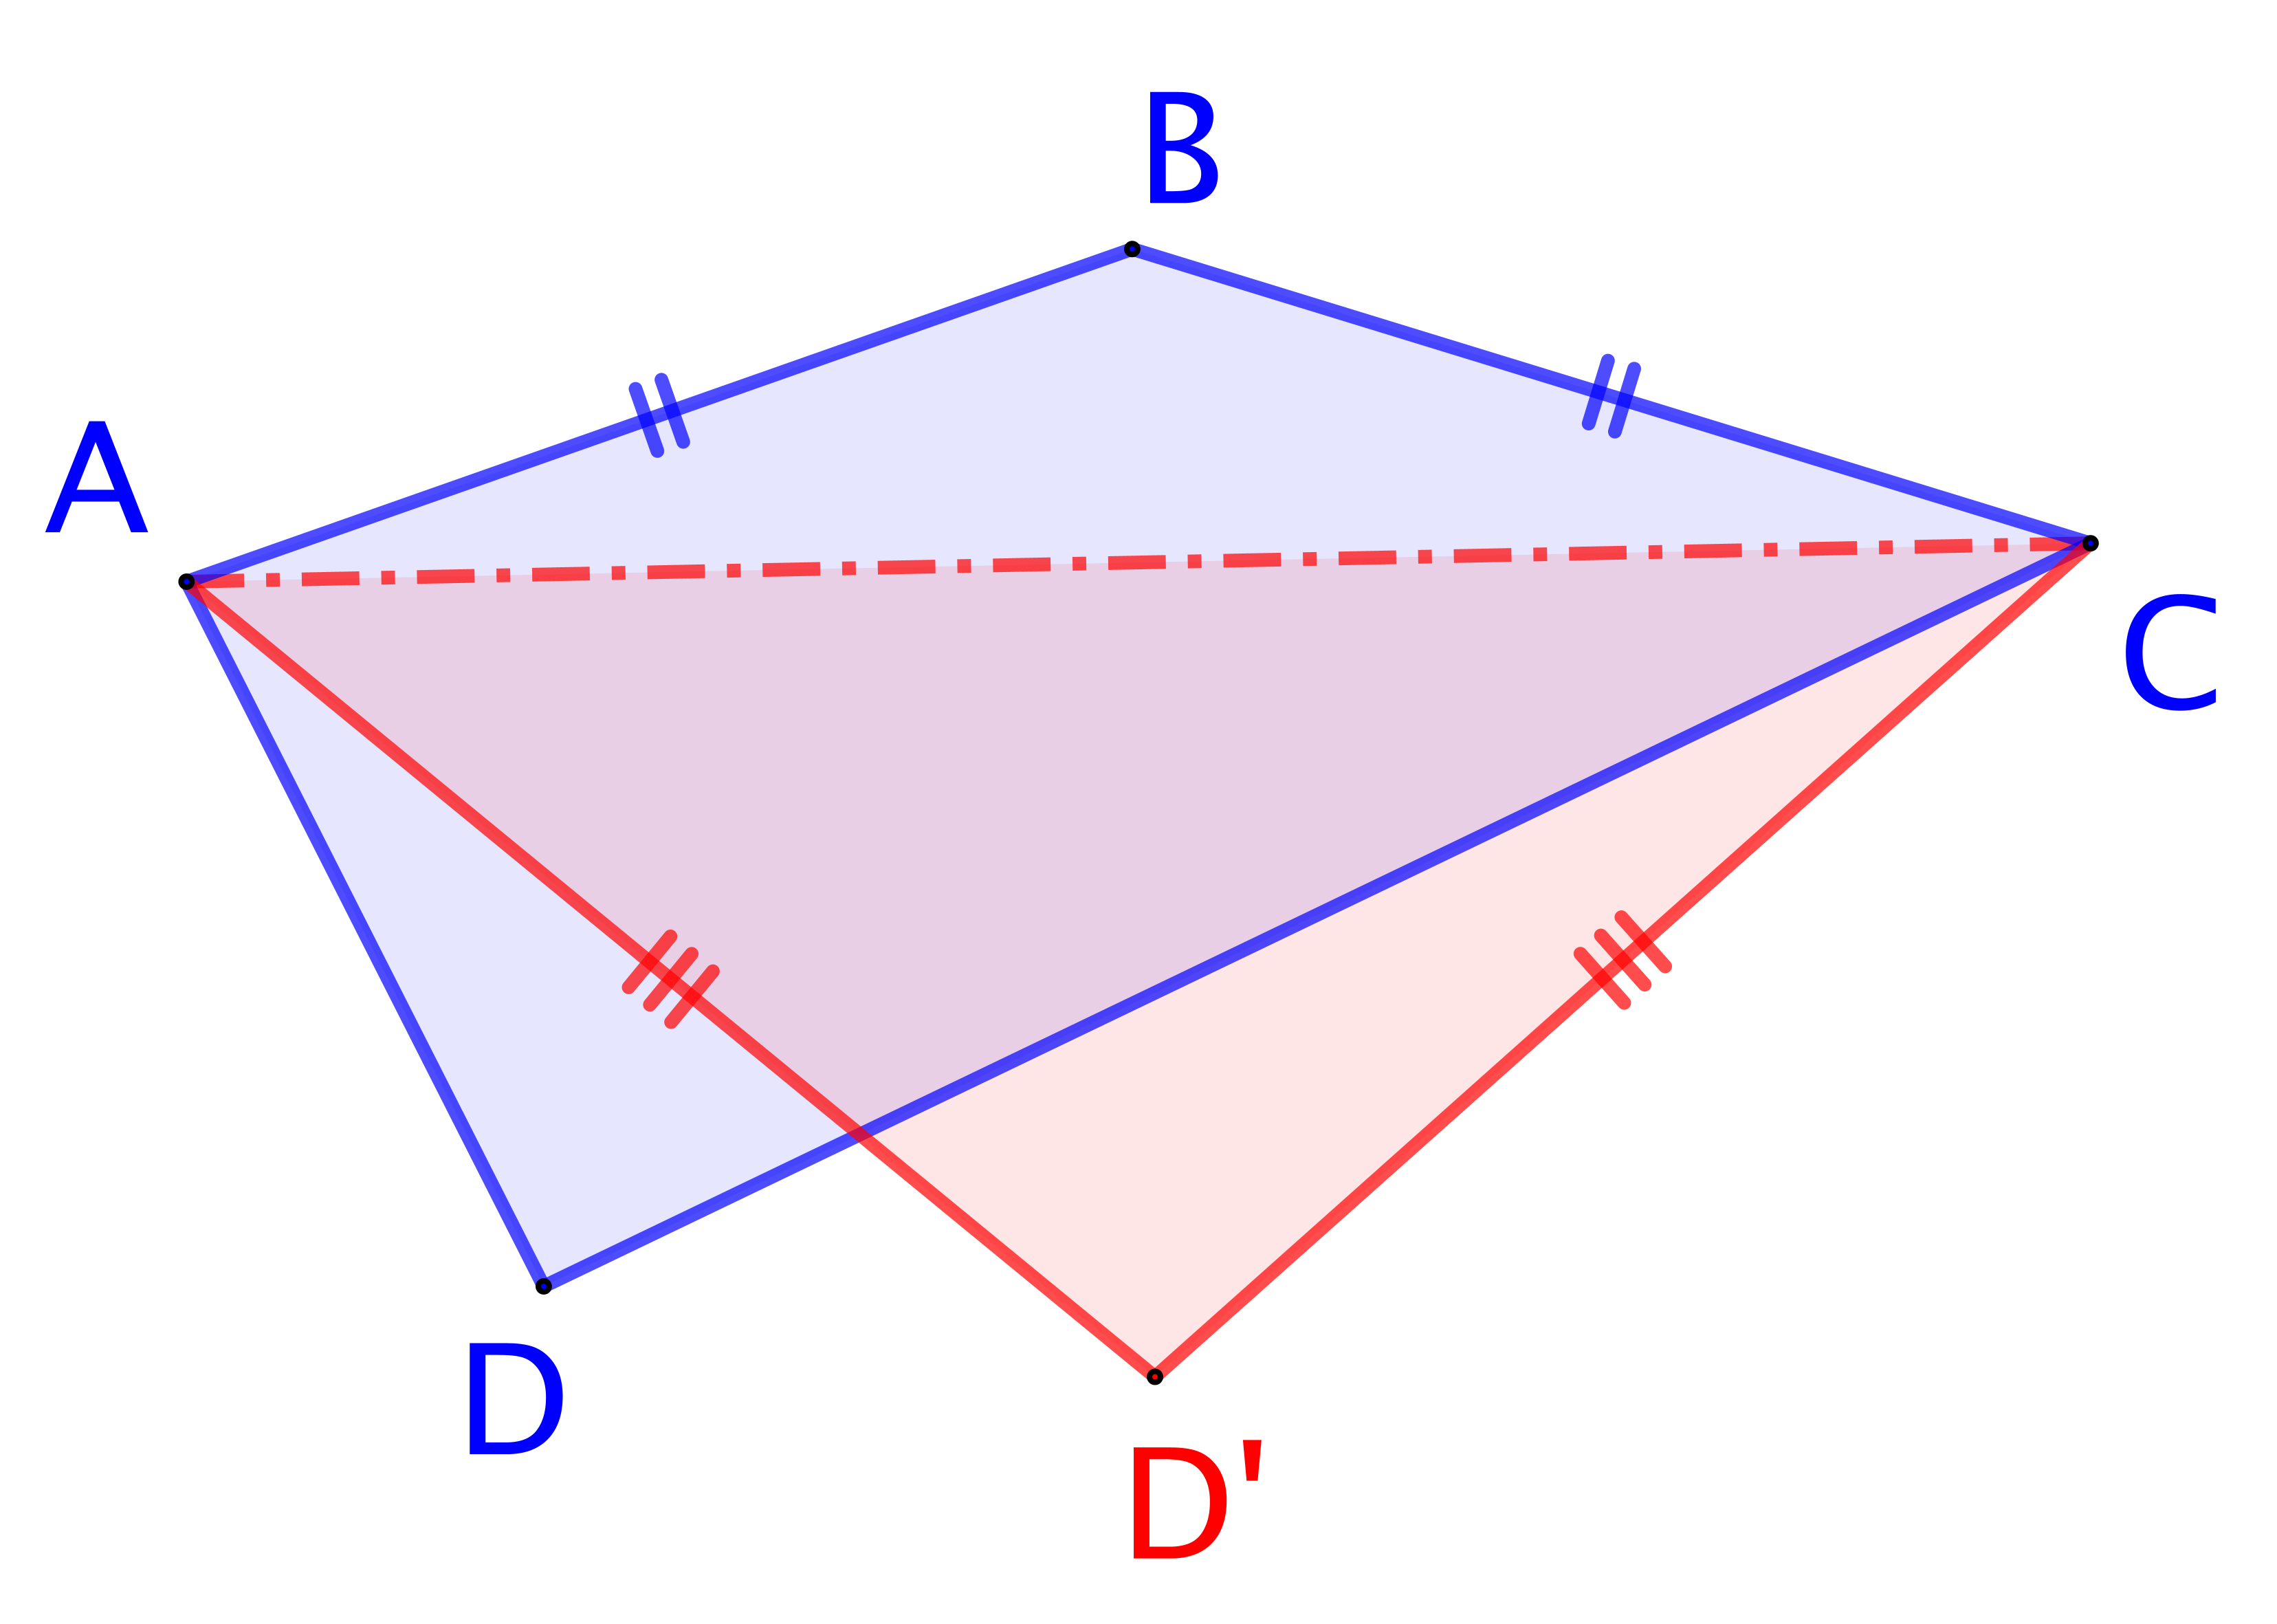
\includegraphics[scale=.4]{convex-one-paire.png}
	\end{center}
	
	
	En supposant que notre cerf-volant ne soit pas un losange, le fait \ref{tri-one-side-fixed} appliqué aux sommets $A$ et $C$ fournit un losange $A^{\,\prime}BC^{\,\prime}D$ de périmètre $p$ vérifiant $\area{A^{\,\prime}BC^{\,\prime}D} > \area{ABCD}$, 
	puisque
	$\num{.5} p = AB + AD$
	et
	$\perim{A^{\,\prime}BD} = \perim{ABD}$
	donnent
	$A^{\,\prime}B = A^{\,\prime}D = \num{.25} p$,
	et de même
	$C^{\,\prime}B = C^{\,\prime}D = \num{.25} p$.

	\begin{center}
		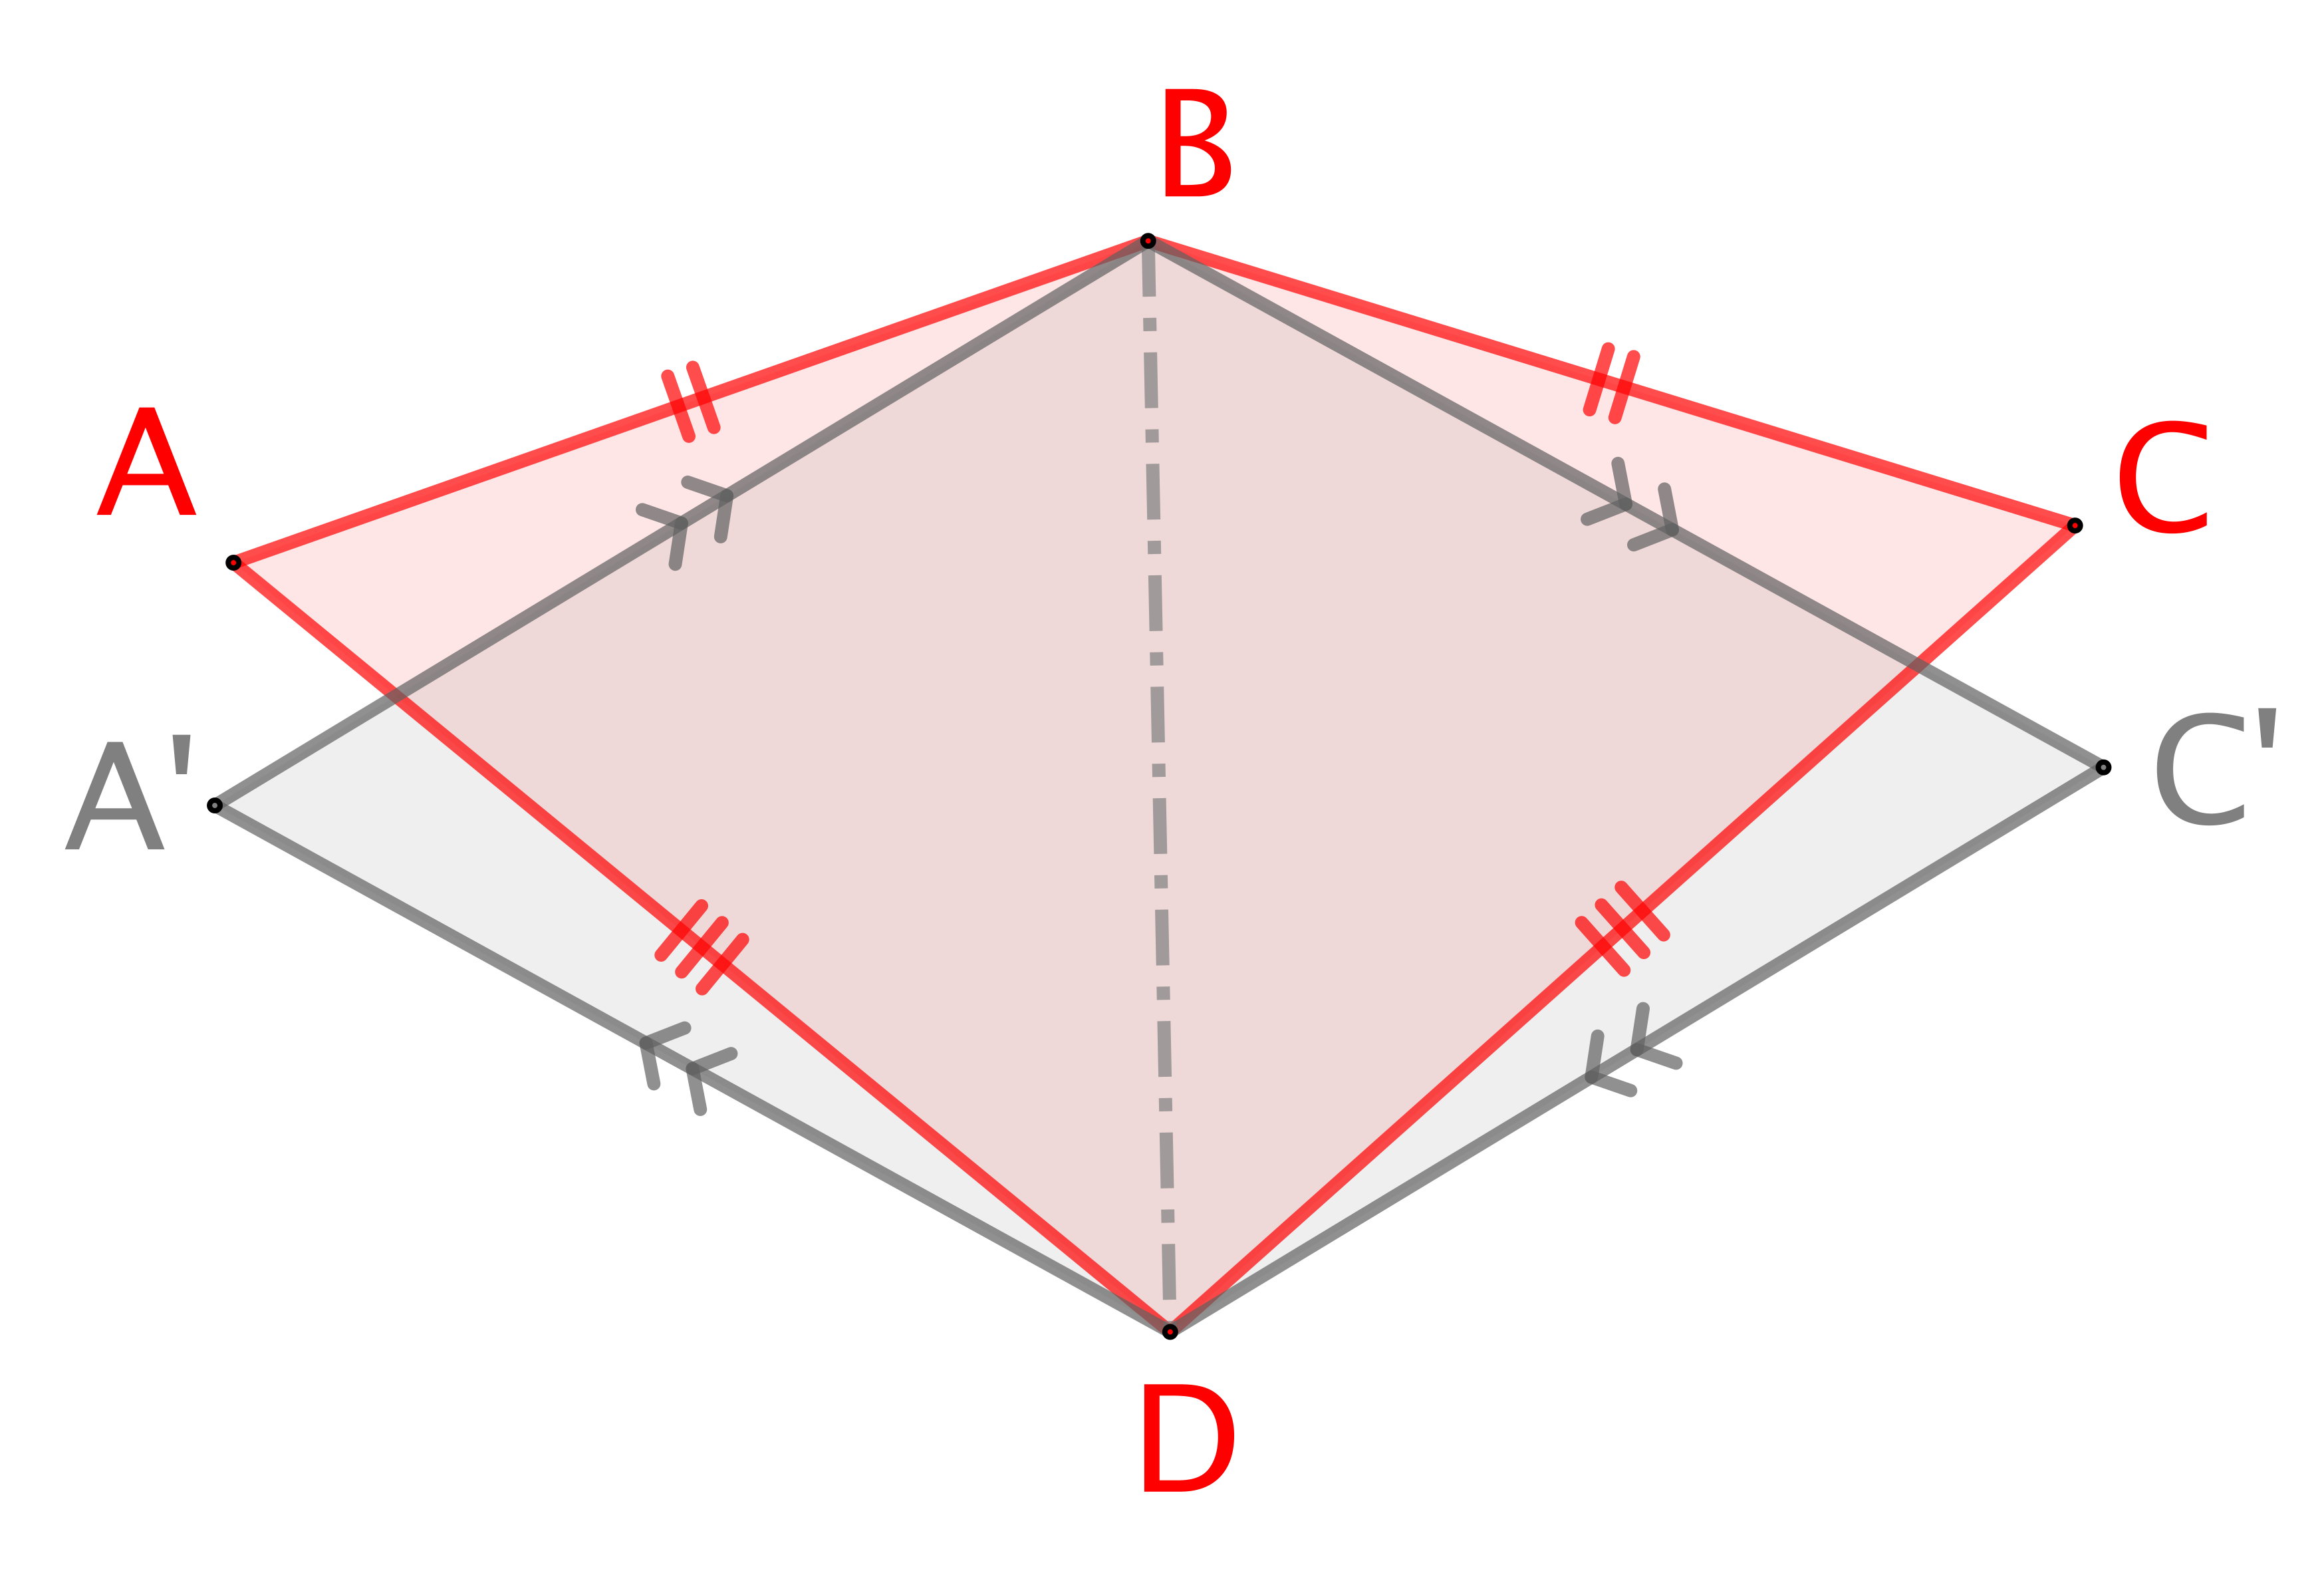
\includegraphics[scale=.4]{convex-isopaire.png}
	\end{center}
	
	
	Pour conclure, il suffit d'appliquer le fait \ref{iso-para}, puisque tout losange est un parallélogramme. Que la géométrie est belle!
\end{proof}


% ----------------------- %


\begin{remark}
	Dans la preuve précédente, nous avons une autre façon de conclure, un peu moins élémentaire.
	%
	En effet, d'après la formule trigonométrique de l'aire d'un triangle,
	un losange $ABCD$ de côté $c$ admet pour aire $c^2 \sin \alpha$ où $\alpha = \anglein{ABC}$.
	Cette aire est donc maximale pour $\anglein{ABC}$ droit, c'est-à-dire lorsque $ABCD$ est un carré.
\end{remark}
